\documentclass[fadttsterUserGuide_master]{subfiles}

\newpage
\begin{document}
	\part{Overview}
		
	\section{Why FADTTSter?}	
	The analysis of brain pathologies and development heavily relies on diffusion tensor imaging (DTI). Conventionally used to map the orientation of the white matter fiber tracts in the brain \citep{dti_brain_mapping1_article,dti_brain_mapping2_article}, DTI uses the isotropic diffusion in cell bodies and spinal fluids and the anisotropic diffusion in axons comprising white matter \citep{dti_article} to assess white matter (WM) integrity and maturation in vivo.
	Functional Analysis of Diffusion Tensor Tract Statistics (FADTTS) is a tool developped to outline the evolution of diffusion properties --- axial diffusivity (AD), radial diffusivity (RD), mean diffusivity (MD) and fractional anisotropy (FA) --- along white matter fiber tracts and their correlation with a set of covariates of interest, such as age or gender \citep{fadtts_article}.
	In the UNC-Utah NA-MIC DTI framework, an end-to-end toolset for atlas fiber tract based DTI analysis, the Matlab (MathWorks Inc, MA, USA) functions implemented in FADTTS \citep{fadtts_manual} are used for the computation of the statistical data \citep{unc-utah_namic_article}.
	However, coding knowledge is necessary to operate it, as the user needs to modify a Matlab script to make it fit each of her/his DTI studies.
	FADTTSter was first created to overcome this issue and make the statistical analysis accessible to any non-technical researcher. Now, FADTTSter is even more developed and features very useful options such as subjects management, profile croping, data plotting, etc.	
		
	\section{What does FADTTSter do?}
	FADTTSter is a user-friendly version of FADTTS designed for users without coding skills. Its aim is to make FADTTS accessible to anyone.
	It can be divided in two major parts, each one working independently.
	\begin{itemize}
		\item \textbf{Matlab script generation:}
		A Matlab script and its mandatory inputs are automatically generated in a folder specific to the ongoing study, based on the information provided by the user (diffusion properties, subjects, qc threshold, nbr of permutations, p-value threshold, etc). Then, if specified, the script can be run on Matlab. 
		\item \textbf{Statistical data plotting:}
		Enables the visualization of the data obtained after running the .m script. The statistical data plotting also allows the user to customized her/his results (tilte, axis, colors, etc).
	\end{itemize}
	FADTTSter is a command line based module as well as a GUI based tool. However, statistical data plotting is only available via the GUI interface.
	\newline
	FADTTSter entirely replaces FADTTS in the UNC-Utah NA-MIC DTI framework, during the statistical analysis of diffusion properties. It uses fiber bundle profiles obtained from \emph{DTIAtlasFiberAnalyzer} \citep{dti_atlas_fiber_analyzer_website} as inputs and \emph{MergeStatWithFiber} \citep{merge_stat_with_fiber_website} can use the outputs for brain visualization.
	\begin{figure}[!h]
		\centering
		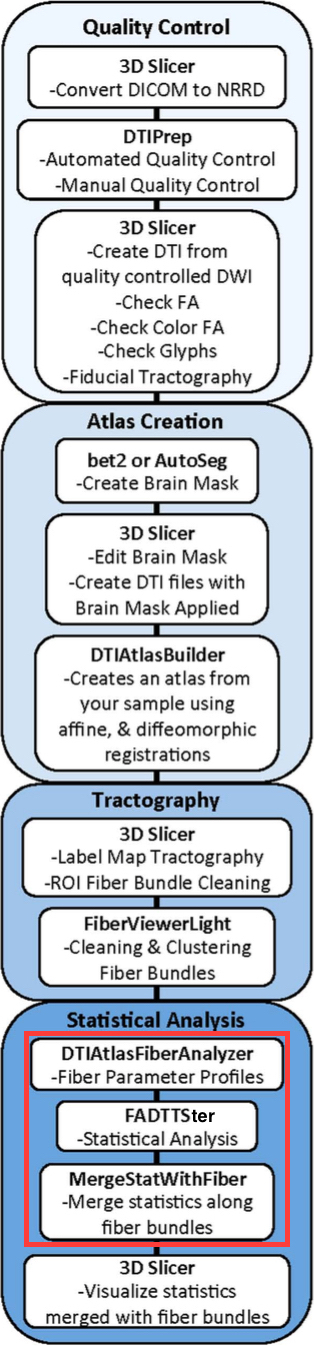
\includegraphics[width=0.25\textwidth]{namicFramework}
		\caption{FADTTSter in the UNC-Utah NA-MIC DTI framework}
		\label{fig:namicFramework}
	\end{figure}
	\newline
	Not only is FADTTSter practical, but it also enables any investigator to perform DTI analysis efficiently.
	\vfill
\end{document}
